\documentclass[10pt, compress]{beamer}
\usetheme[conference=TCV-Topic21 KoM,venue=Lausanne, date=15/05/2017, titleprogressbar, logo=RFX-logo]{Eurof}
\usepackage{listings,amsmath,multimedia, amssymb}
\usepackage{../beamerclass/tangocolors}
\usepackage{../beamerclass/rfxcolor}
% for drawing
\usepackage{pgf}
\usepackage{tikz}
\usetikzlibrary{arrows,shapes,backgrounds}
\usepackage{../beamerclass/onimage}
\usepackage[export]{adjustbox}
\usepackage{bm}
% for font
\usepackage[absolute,overlay]{textpos}
  \setlength{\TPHorizModule}{1mm}
  \setlength{\TPVertModule}{1mm}

\usepackage[style=nature,citestyle=authoryear-comp,defernumbers=true,maxnames=2,firstinits=true,
uniquename=init,backend=bibtex8,arxiv=abs,mcite]{biblatex}
\bibliography{biblio}
\renewcommand*{\bibfont}{\footnotesize}
\renewcommand*{\citesetup}{\footnotesize}
\usepackage[export]{adjustbox}
\makeatother
\mode<presentation>
\makeatletter
% add a macro that saves its argument
\newcommand{\footlineextra}[1]{\gdef\insertfootlineextra{#1}}
\newbox\footlineextrabox
% for reducing font on a single slide
\newcommand\Fontvi{\fontsize{8}{7.2}\selectfont}
\title{Topic 21 experiment Week 24}
\date{26 June 2017}
\author[Topic 21 ST]{N . VianTllo and V. Naulin for the
  Topic 21 SC team}
\begin{document}
\tikzstyle{every picture}+=[remember picture]
\maketitle
\begin{frame}{Scientific Team}
  \begin{description}
  \item[EPFL:] H. De Oliveira, R. Maurizio, B. Labit,
    C. Tsui, K. Verhaegh, H. Reimerdes, C. Theiler
  \item[DTU:] J.J. Rasmussen and V. Naulin
  \item[RFX:] N. Vianello, M. Spolaore, M. Agostini
  \item[OEAW:] B. Schneider, S. Costea, R. Schrittwieser
  \item[CCFE:] F. Militello
  \item[JSI:] J. Kovacic
  \end{description}
\end{frame}
\begin{frame}{TCV experiments: boundary condition}
\vspace{-1cm}
\Fontvi
\begin{itemize}
\item 2017 \textbf{objectives} listed after the General Planning Meeting
  \begin{enumerate}
  \item Provide cross-machine \alert{L-Mode} shoulder dependence on
    current both at constant Bt and at constant q$_{95}$
  \item Establish robust scenario for density shoulder profile in
        H-mode and establish dependence on fuelling/neutral
        profiles/divertor condition
  \item Study the role of ELM regimes, neutral compression, and
    particle density in filamentary transport and related shoulder
    formation.
  \item Identify the contribution of collisionality and
    seeding on filamentary transport and related shoulder
    formation.
  \item Determine the effect of filaments and shoulder
    formation on target heat loads in different Hmode plasmas.
  \end{enumerate}
\item We have a total number of \textbf{\# 23 Shots} originally split into two
    operational window. Calendar week 24 (12.06-16.06) and Calendar
    week 43 (23.10-27.10)
\end{itemize}
\end{frame}

\begin{frame}{Experimental plan}
\Fontvi
    \alert{For the first week of operation we originally planned L-mode shots
      only. Shots 1-3 I$_p$ scan at constant toroidal field. Shots
      1, 4 and 5 I$_p$ scan at constant q$_{95}$ to be compared with
      analogous experiments in AUG and MAST-U. Shots 6-7 Low
      collisionality scan. Shots 8-9 DN current scan: this will be
      compared directly with Mast-U which will run predominantly in DN
    configuration. Shot 10-11 Current scan in forward field to check
    the role of $\nabla\times B$ direction.}
\begin{enumerate}
\item Shape from 57088, I$_p$ = 245 kA,  Reverse B$_t$,
    density ramp from Line Average Density = 3.8e19 @ 0.5 s to 11e19 @ 1.6s,  Bt = 1.4T. Plunge @ 0.65, 1.52
\item  Repeat \# 1 with I$_p$=330 kA Bt=1.4T, same density ramp, same timing for plunges
\item  Repeat \# 1 with I$_p$=180 kA, Bt=1.4T, same density ramp, same timing for plunges
\item  Repeat \# 1 with q95=2.44 as \# 2, adjust Bt consequently (Bt = 1.02T)
\item  Repeat \# 3 with q95=2.44 as \# 2, adjust Bt consequently (Bt=0.8T)
\item  Shape and current from \# 1. Stop puffing once the divertor is
  formed to get low collisionality case. ECRH ramp from 0.9s (150
  kW--500 kW)
\item  Repeat \# 6 with intermediate density value between \# 6 and
  \#1 density at 0.65s. 
\item  Repeat density ramp of Shot \# 2 in DN configuration 
\item  Repeat density ramp of Shot \# 3 in DN configuration 
\item Repeat \# 1 in forward field
\item Repeat \# 3 in forward field
\end{enumerate}
\end{frame}

\begin{frame}{Current scan at constant B$_{\phi}$}
\Fontvi
  \begin{columns}[c]
    \begin{column}{0.7\textwidth}
      \includegraphics<1>[width=8.cm]{../../Experiments/TCV/analysis/pdfbox/CurrentScanConstantBt}
      \includegraphics<2>[width=8.cm]{../../Experiments/TCV/analysis/pdfbox/DensityProfileCurrentScanConstantBtSOL}
      \includegraphics<3>[width=8.cm]{../../Experiments/TCV/analysis/pdfbox/DensityProfileCurrentScanConstantBt}
    \end{column}
    \begin{column}{0.3\textwidth}
      \begin{itemize}
        \item Confirming results from Topic-25 increasing the current
          reduces the ion flux rollover density threshold
        \item Neutral compression seems slightly reduced at higher current
        \item<2-> Profiles from RCP are not yet clear, with the only
          robust variation between 245 and 330 kA
        \item<3-> If we combine with Thomson scattering there are still
          unresolved issue
        \end{itemize}
    \end{column}
  \end{columns}
\end{frame}

\begin{frame}{Current scan at constant q$_{95}$}
\Fontvi
  \begin{columns}[c]
    \begin{column}{0.7\textwidth}
      \includegraphics<1>[width=8.cm]{../../Experiments/TCV/analysis/pdfbox/CurrentScanConstantQ95}
      \includegraphics<2>[width=8.cm]{../../Experiments/TCV/analysis/pdfbox/DensityProfileCurrentScanConstantQ95SOL}
      \includegraphics<3>[width=8.cm]{../../Experiments/TCV/analysis/pdfbox/DensityProfileCurrentScanConstantQ95}
    \end{column}
    \begin{column}{0.3\textwidth}
      \begin{itemize}
        \item Unusual scenarios with B$_{phi}$ up to 0.8T. \alert{No rollover
          on at any of the current}
        \item Expected higher target neutral pressure increase at
          higher current
        \item<2-> Profiles from RCP suggest slight flattening in the
          far SOL at higher current
        \item<3-> Confirmed even combining with Thomson data
        \end{itemize}
    \end{column}
  \end{columns}
\end{frame}
\begin{frame}{Attempt for low collisionality}
  \begin{columns}[c]
    \begin{column}{0.7\textwidth}
      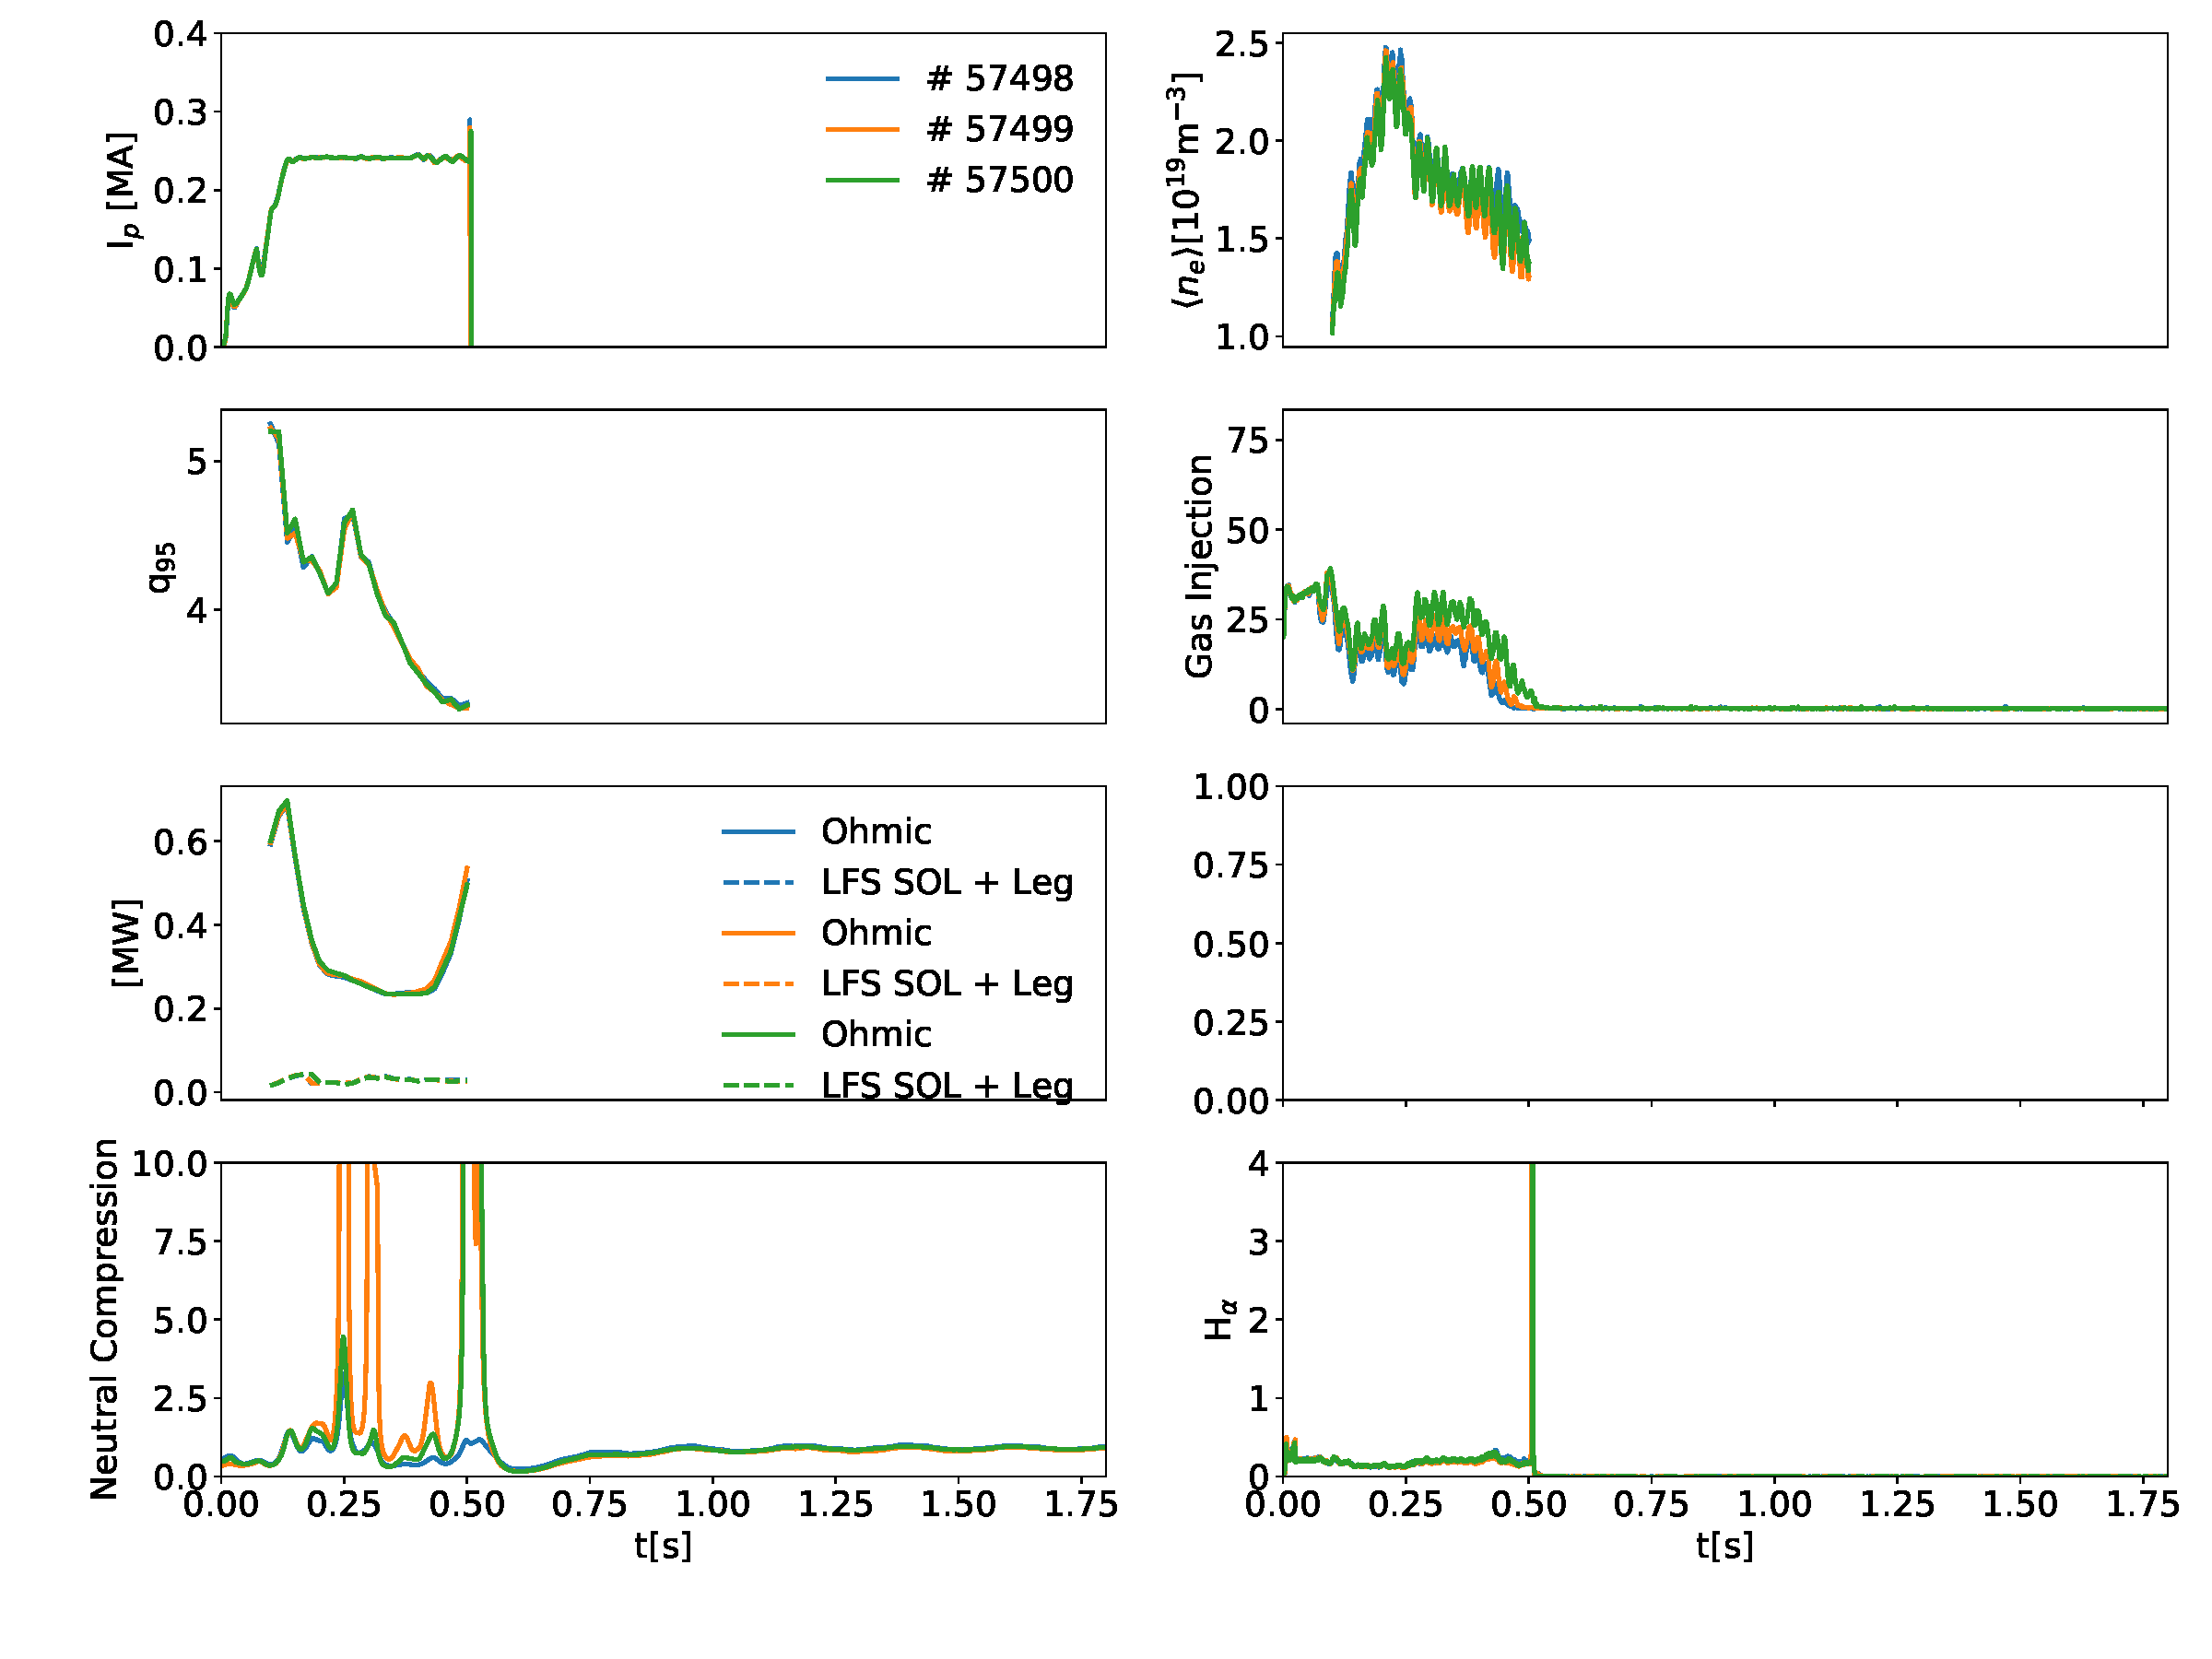
\includegraphics[width=8.cm]{../../Experiments/TCV/analysis/pdfbox/LowCollisionalityAttempt}
    \end{column}
    \begin{column}{0.3\textwidth}
      All the attempt to perform a low collisionality case disrupted
      whenever density decreases below a certain threshold
    \end{column}
  \end{columns}
\end{frame}

\begin{frame}{Conclusion}
  \Fontvi
\begin{enumerate}
\item \textcolor{green}{Shape from 57088, I$_p$ = 245 kA,  Reverse B$_t$,
    density ramp from Line Average Density = 3.8e19 @ 0.5 s to 11e19 @ 1.6s,  Bt = 1.4T. Plunge @ 0.65, 1.52}
\item  \textcolor{green}{Repeat \# 1 with I$_p$=330 kA Bt=1.4T, same density ramp, same timing for plunges}
\item  \textcolor{green}{Repeat \# 1 with I$_p$=180 kA, Bt=1.4T, same density ramp, same timing for plunges}
\item  \textcolor{green}{Repeat \# 1 with q95=2.44 as \# 2, adjust Bt consequently (Bt = 1.02T)}
\item  \textcolor{green}{Repeat \# 3 with q95=2.44 as \# 2, adjust Bt consequently (Bt=0.8T)}
\item  \textcolor{red}{Shape and current from \# 1. Stop puffing once the divertor is
  formed to get low collisionality case. ECRH ramp from 0.9s (150
  kW--500 kW)}
\item  \textcolor{red}{Repeat \# 6 with intermediate density value between \# 6 and
  \#1 density at 0.65s.} 
\item  \textcolor{red}{Repeat density ramp of Shot \# 2 in DN configuration} 
\item  \textcolor{red}{Repeat density ramp of Shot \# 3 in DN configuration} 
\item \textcolor{red}{Repeat \# 1 in forward field}
\item \textcolor{red}{Repeat \# 3 in forward field}
\end{enumerate}

\end{frame}

\end{document}

